\chapter{Analisis}
\label{chap:analisis}

Pada bab ini akan dijelaskan analisis yang telah dilakukan terhadap \textit{privacy preserving data mining}, teknik randomisasi, studi kasus, teknik penambangan data, dan gambaran umum perangkat lunak. Perancangan perangkat lunak akan dijelaskan melalui diagram aktivitas dan diagram kelas yang telah dibuat berdasarkan analisis yang telah dilakukan.

\section{Analisis Masalah}
\label{sec:analisis-masalah}

Pada penelitian ini masalah yang ingin dicoba untuk diselesaikan adalah privasi yang terlanggar tidak sebanding dengan hasil yang didapatkan pada penambangan data. Privasi pada data yang digunakan untuk proses penambangan data mungkin saja didapatkan oleh pihak yang tidak berhak. Oleh karena itu, penelitian ini menguji salah satu solusi terhadap masalah tersebut dengan cara mengacak data yang akan ditambang dengan metode \textit{Randomization} sehingga privasinya hilang tetapi data tersebut tetap dapat digunakan untuk penambangan data. Privasi yang perlu dijaga antara lain mengenai identitas seseorang atau hal yang dapat dikaitkan terhadap identitas seseorang. Dua buah teknik yang digunakan yaitu \textit{Random Rotation Perturbation} dan \textit{Random Projection Perturbation} akan diimplementasikan menjadi perangkat lunak dan akan diuji kualitas dari hasil teknik tersebut dengan melakukan penambangan data.

\subsection{Implementasi Metode \textit{Randomization}}
\label{subsec:analisis-ppdm}

Teknik yang dipilih untuk diimplementasikan adalah teknik \textit{Random Rotation Perturbation} dan \textit{Random Projection Perturbation}. Tetapi ada kekurangan pada kedua teknik tersebut yaitu nilai setiap data yang ingin dirandomisasi harus bersifat numerik dan kedua teknik tersebut hanya menjaga jarak Euclidean antara setiap titik (sebuah baris pada dataset) dengan titik lainnya sehingga hanya teknik penambangan data yang bergantung pada jarak Euclidean saja yang dapat digunakan. Oleh karena itu, kedua teknik randomisasi akan diuji dengan melakukan penambangan data dengan teknik klasifikasi yaitu \textit{k-nearest neighbors} dan teknik \textit{clustering} yaitu \textit{k-means} untuk menguji coba keberhasilan kedua teknik randomisasi dan untuk membandingkan kualitas hasil dari kedua teknik randomisasi tersebut.

Perangkat lunak diharapkan dapat berfungsi untuk menerapkan teknik \textit{Random Rotation Perturbation} terhadap dataset apapun dengan syarat seluruh fiturnya bersifat numerik dan menerapkan teknik \textit{Random Projection Perturbation} terhadap dataset yang memenuhi persyaratan yaitu dimensinya cukup besar dan seluruh fiturnya bersifat numerik. Hasil akhir dari perangkat lunak akan berbentuk sebuah dokumen berjenis \textit{comma-separated values}. Pada penambangan data, sebuah model yang telah dibuat sangat mungkin untuk dilatih lagi dengan data yang baru. Oleh karena itu, perangkat lunak juga diharapkan dapat menyimpan matriks rotasi/proyeksi yang telah dibuat agar dapat digunakan kembali apabila ada penambahan data di waktu yang akan datang.

Metode \textit{Randomization} akan diimplementasikan dengan bantuan bahasa pemograman Python beserta berbagai \textit{library} seperti Pandas, Numpy, Scikit-learn, dan Scipy. Perangkat lunak randomisasi akan dibangun beserta antarmukanya dengan bantuan \textit{framework} antarmuka yaitu Kivy.

\subsubsection{Teknik \textit{Random Rotation Perturbation}}
\label{subsubsec:analisis-rrp}

Teknik \textit{Random Rotation Perturbation} menggunakan matriks orthogonal untuk mengacak dataset tanpa mengubah jarak Euclidean dataset tersebut. Matriks orthogonal relatif sulit dibuat pada dimensi yang tinggi dan kompleksitasnya tidak kecil yaitu \(O(n^2)\)~\cite{stewart:80:orthogonal}. Untuk dataset yang sangat besar, masih dapat dilakukan randomisasi dengan teknik ini walaupun mungkin akan sedikit memakan waktu. Hal ini akan diuji pada bab 5 saat pengujian eksperimental.

Walaupun seperti itu, teknik ini dapat menjamin bahwa tidak akan ada distorsi yang terjadi pada jarak Euclidean pada seluruh data atau dengan kata lain jarak Euclideannya tidak berubah sama sekali. Hal ini disebabkan oleh metode yang dipakai hanya dengan merotasi seluruh titik yang merepresentasikan sebuah objek data dalam bidang Euclidean. Transformasi rotasi akan merubah nilai setiap titik pada bidang tersebut tetapi karena pada dasarnya setiap titik bergerak dengan gerakan yang sama yaitu sebuah rotasi yang sama sehingga tidak akan ada perubahan pada jarak Euclidean antara seluruh titik-titik yang ada.

Transformasi rotasi mempunyai kelemahan yaitu apabila ada titik pada bidang Euclidean yang nilainya kecil mendekati 0 maka walaupun dirotasi dengan rotasi yang berbeda-beda, bagaimanapun juga titik tersebut akan tetap bernilai kecil atau berada dekat dengan nilai 0. Hal ini berpotensi menjadi sebuah faktor yang lemah untuk melindungi privasi~\cite{rotation:05:chenliu}. Oleh karena itu tranformasi translasi perlu dilakukan sebelum melakukan rotasi agar titik tersebut tidak selalu mendekati nilai 0 saat dirotasi dengan berbagai macam rotasi. Transformasi translasi akan dilakukan dengan melakukan translasi yang nilainya diambil secara acak pada rentang [0, 100] sehingga translasi yang dilakukan tidak bisa diketahui oleh orang yang tidak berhak.

\subsubsection{Teknik \textit{Random Projection Perturbation}}
\label{subsubsec:analisis-projection}

Teknik \textit{Random Projection Perturbation} didasarkan pada lemma \textit{Johnson-Lindenstrauss} yang mengatakan bahwa sejumlah titik pada bidang Euclidean berdimensi tertentu dapat diproyeksikan ke dimensi yang lebih kecil tanpa mengubah secara signifikan jarak Euclidean antara titik-titik tersebut. \textit{Error} terburuk yang dapat terjadi pada jarak Euclidean setelah proyeksi diterapkan ditentukan oleh nilai variabel \textit{epsilon} dengan pertidaksamaan sebagai berikut menunjukkan rentang jarak Euclidean sebuah objek data setelah diproyeksi.
\begin{equation}
	(1-eps)||u - v||^{2}<||p(u) - p(v)||^{2}<(1+eps)||u - v||^{2}
\end{equation}
Pertidaksamaan di atas menyatakan bahwa kuadrat dari jarak Euclidean antara dua buah titik setelah diproyeksi tidak akan kurang dari kuadrat jarak Euclidean aslinya dikalikan \((1-eps)\) dan tidak akan lebih dari kuadrat jarak Euclidean aslinya dikalikan \((1+eps)\). Lemma \textit{Johnson-Lindenstrauss} menjamin bahwa jarak Euclidean pada data setelah diproyeksi hanya akan berada pada rentang tersebut dan bisa saja jarak Euclidean setelah diproyeksi sangat dekat dengan jarak Euclidean aslinya karena belum tentu jarak Euclidean data setelah diproyeksi menyentuh batas pertidaksamaan tersebut. Tetapi pertidaksamaan ini juga dapat menyatakan bahwa jarak Euclidean setelah diproyeksi dengan aslinya tidak mungkin sama persis.

Agar pertidaksamaan sebelumnya berlaku ada persyaratan yang harus dipenuhi yaitu nilai minimal variabel \(k\) atau dengan kata lain target dimensi terkecilnya proyeksi dilakukan harus memenuhi persamaan berikut.
\begin{equation}
	k \geq 4(\epsilon^{2}/2-\epsilon^{3}/3)^{-1}\ln{n}
\end{equation}
Variabel \(n\) pada persamaan tersebut adalah jumlah titik pada bidang Euclidean atau dengan kata lain jumlah baris pada dataset yang ingin dirandomisasi. Dengan melihat persamaan tersebut maka bisa disimpulkan bahwa dimensi minimal sebuah dataset diproyeksikan berbanding lurus dengan jumlah baris pada dataset tersebut. Apabila sebuah dataset diproyeksikan ke dimensi paling minimal dan diterapkan teknik penambangan data sehingga menghasilkan sebuah model penambangan data dengan data latihannya adalah dataset tersebut maka model tersebut akan melanggar persamaan di atas jika model tersebut dilatih kembali dengan data yang baru karena artinya bidang Euclidean yang disebutkan tadi akan memiliki titik yang lebih banyak, nilai \(n\) yang lebih besar. 

Oleh karena itu, berdasarkan analisis di atas teknik \textit{Random Projection Perturbation} tidak relevan untuk model penambangan data yang memiliki sangat banyak data tetapi berdimensi relatif kecil dibandingkan dengan jumlah datanya. Tetapi masalah ini dapat dihindari dengan tidak mereduksi dimensi ke dimensi yang sangat kecil atau paling minimal sehingga tidak terlalu cepat nilai minimal variabel \(k\) meningkat sampai menyusul dimensi dataset setelah proyeksi. Selain itu, jarak Euclidean setelah diproyeksi juga belum tentu pasti menyentuh batas pertidaksamaan yang di atas sehingga belum tentu hasil randomisasi memiliki distorsi yang sangat besar apabila besar dimensi melebihi nilai minimal variabel \(k\). Hal ini akan diuji pada bab 5 saat melakukan pengujian eksperimental.

Teknik \textit{Random Projection Perturbation} memiliki kompleksitas yang relatif kecil yaitu \(O(dkn)\) ~\cite{bingham:01:projection}. Dengan kompleksitas yang cukup rendah maka teknik ini dapat bekerja secara cepat untuk penambangan data dengan dataset yang besar sekalipun. Oleh karena itu, teknik ini berpotensi dapat berkerja dengan baik dalam lingkungan \textit{big data} karena kompleksitas yang relatif kecil dan dapat bekerja pada dataset yang sangat besar. Hal ini disebabkan oleh metode yang digunakan oleh teknik ini adalah melakukan proyeksi dengan cara mengkalikan dataset yang sudah berbentuk matriks dengan matriks proyeksi yang berupa matriks acak saja, tidak ada sifat spesial pada matriks acak tersebut seperti teknik \textit{Random Rotation Perturbation} sehingga pembuatan matriks proyeksinya dapat dilakukan dengan cepat.

\subsection{Pengujian Dengan Penambangan Data}
\label{subsec:analisis-penambangan}

Pengujian fungsional dan eksperimental akan dilakukan masing-masing untuk menguji apakah perangkat lunak berfungsi secara benar menerapkan metode \textit{Randomization} dan menguji hasil perangkat lunak. Pengujian fungsional dilakukan dengan membandingkan nilai pada dataset asli dan dataset yang telah dirandomisasi apakah berbeda. Pengujian eksperimental dilakukan untuk melihat perbedaan apa saja yang terjadi pada dataset. Pengujian tersebut membandingkan beberapa informasi pada dataset yaitu rata-rata, standar deviasi, nilai terkecil dan terbesar pada sebuah kolom, kuartil bawah, kuartil tengah, dan kuartil atas. Selain itu pada pengujian eksperimental akan membandingkan model penambangan data klasifikasi dan \textit{clustering} antara model yang dilatih menggunakan dataset asli dan dataset yang telah dirandomisasi.

Teknik penambangan data akan diimplementasikan dengan bantuan bahasa pemograman Python beserta berbagai \textit{library} seperti Pandas, Numpy, Scikit-learn, dan Scipy. Perangkat lunak untuk menerapkan penambangan data akan dijalankan dengan bantuan perangkat lunak Spyder dan Anaconda untuk menampilkan visualisasi dan teks yang dihasilkan oleh perangkat lunak penambangan data yang berbahasa pemograman Python. 

\subsubsection{Pengujian Dengan Teknik Penambangan Data Klasifikasi \textit{K-nearest Neighbors}}
\label{subsubsec:analisis-knn}

Teknik penambangan data klasifikasi yang digunakan untuk menguji kualitas hasil dari metode \textit{Randomization} adalah teknik \textit{k-nearest neighbors}. Hasil dari metode \textit{Randomization} diharapkan masih dapat digunakan untuk penambangan data klasifikasi dengan kualitas yang sama seperti memakai dataset (asli) yang tidak dirandomisasi. Pada pengujian yang akan dilakukan, perbandingan antara dataset asli dengan dataset yang telah dirandomisasi akan dilakukan dengan melakukan proses dari awal sampai akhir pembuatan model klasifikasi hingga evaluasi model tersebut. Tujuan utama pengujian adalah membandingkan akurasi (dalam memprediksi \textit{test set}) terbaik model yang dibuat dengan dataset asli dan dataset yang telah dirandomisasi. Apabila akurasi tersebut sama atau mirip, maka teknik randomisasi yang digunakan dapat dinyatakan berhasil dan efektif digunakan untuk \textit{privacy preserving data mining} dengan teknik penambangan data klasifikasi menggunakan algoritma \textit{k-nearest neighbors}.

Dataset asli dan dataset yang telah dirandomisasi masing-masing akan digunakan untuk membuat model \textit{k-nearest neighbors}. Proses penambangan data \textit{k-nearest neighbors} dilakukan dengan langkah-langkah berikut ini.
\begin{enumerate}
    \item Membuat 20 (dapat berubah disesuaikan dengan pengujian yang dilakukan) model \textit{k-nearest neighbors} dengan nilai variabel \textit{k} sebesar 1 sampai 20 untuk mengetahui model dengan nilai variabel \textit{k} mana yang memiliki akurasi tertinggi
    \item Melatih 20 model tersebut dengan \textit{training set} (60 persen baris pada dataset diambil secara acak) yang sama
    \item Melakukan prediksi dengan 20 model tersebut terhadap \textit{training set} yang sama
    \item Melakukan prediksi dengan 20 model tersebut terhadap \textit{test set} (40 persen baris pada dataset diambil secara acak) yang sama
    \item Menghitung akurasi 20 model tersebut pada hasil prediksi \textit{training set} dan \textit{test set}
    \item Membuat grafik hubungan antara nilai variabel \textit{k} dengan akurasi pada \textit{training set} dan \textit{test set}
    \item Menampilkan seluruh nilai akurasi pada setiap nilai variabel \textit{k}
    \item Membuat model dengan nilai variabel \textit{k} yang memiliki akurasi tertinggi lalu menghitung akurasinya pada \textit{test set} dan menghitung waktu eksekusi saat melatih model dan melakukan prediksi
    \item Menampilkan akurasi model, waktu eksekusi untuk melatih model, dan waktu eksekusi dalam melakukan prediksi dengan model tersebut
\end{enumerate}
Proses penambangan data tersebut dilakukan dua kali masing-masing menggunakan dataset asli dan dataset yang telah dirandomisasi agar dapat dibandingkan nilai akurasi tertinggi, nilai variabel \textit{k} yang memiliki akurasi tertinggi, dan waktu eksekusi pelatihan model dan prediksi dengan model tersebut. Dengan membandingkan akurasi model dapat diketahui apakah metode \textit{Randomization} yang digunakan mempunyai kualitas yang baik atau tidak untuk digunakan dalam penambangan data klasifikasi dengan teknik \textit{k-nearest neighbors}. Kedua model klasifikasi yang dibandingkan dapat dinyatakan sama atau mirip apabila akurasi masing-masing pada kedua model tersebut mempunyai nilai yang sama atau tidak jauh perbedaannya.

\subsubsection{Pengujian Dengan Teknik Penambangan Data \textit{Clustering} \textit{K-means}}
\label{subsubsec:analisis-kmeans}

Teknik penambangan data \textit{clustering} yang digunakan untuk menguji kualitas hasil dari metode \textit{Randomization} adalah teknik \textit{k-means}. Hasil dari metode \textit{Randomization} diharapkan masih dapat digunakan untuk penambangan data \textit{clustering} dengan kualitas yang sama seperti memakai dataset (asli) yang tidak dirandomisasi. Pada pengujian yang akan dilakukan, perbandingan antara dataset asli dengan dataset yang telah dirandomisasi akan dilakukan dengan melakukan proses dari awal sampai akhir pembuatan model \textit{clustering} hingga evaluasi model tersebut. Tujuan utama pengujian adalah membandingkan jumlah \textit{cluster} yang ada dan anggota pada tiap \textit{cluster} apakah sama atau mirip pada dataset asli dan dataset yang telah dirandomisasi. Apabila jumlah \textit{cluster}-nya sama dan anggota-anggota tiap \textit{cluster} sama atau mirip, maka teknik randomisasi yang digunakan dapat dinyatakan berhasil dan efektif digunakan untuk \textit{privacy preserving data mining} dengan teknik penambangan data \textit{clustering} menggunakan algoritma \textit{k-means}.

Perlu diperhatikan bahwa teknik \textit{Random Projection Perturbation} memiliki persyaratan yaitu dataset yang digunakan harus berdimensi cukup besar. Hal ini membuat visualisasi sulit untuk dilakukan, oleh karena itu teknik \textit{Principal Component Analysis} digunakan untuk mereduksi dimensi dataset yang sangat besar dalam pengujian ini menjadi 2 dimensi saja. Teknik ini sudah terbukti relatif baik dan sudah umum digunakan untuk teknik penambangan data \textit{clustering} dengan algoritma \textit{k-means}.

Dataset asli dan dataset yang telah dirandomisasi masing-masing akan digunakan untuk membuat model \textit{k-means}. Proses penambangan data \textit{k-means} dilakukan dengan langkah-langkah berikut ini.
\begin{enumerate}
    \item Membuat 9 model \textit{k-means} dengan nilai variabel \textit{k} sebesar 2 sampai 10 untuk mengetahui model dengan nilai variabel \textit{k} mana yang memiliki \textit{cluster} terbaik
    \item Melatih 9 model tersebut dengan dataset yang sama
    \item Menghitung nilai \textit{Sum of Squared Error} dan \textit{Silhoutte Score} pada 9 model tersebut
    \item Membuat grafik hubungan antara nilai variabel \textit{k} dengan nilai \textit{Sum of Squared Error}
    \item Membuat grafik hubungan antara nilai variabel \textit{k} dengan nilai \textit{Silhoutte Score}
    \item Menampilkan seluruh nilai \textit{Sum of Squared Error} pada setiap nilai variabel \textit{k}
    \item Menampilkan seluruh nilai \textit{Silhoutte Score} pada setiap nilai variabel \textit{k}
    \item Menampilkan nilai \textit{Silhoutte Score} tertinggi dan nilai variabel \textit{k}-nya
    \item Membuat model dengan nilai variabel \textit{k} yang memiliki \textit{Silhoutte Score} tertinggi lalu menghitung \textit{Silhoutte Score}-nya dan menghitung waktu eksekusi saat melatih model
    \item Menampilkan visualisasi \textit{cluster} pada model dengan \textit{Scatter Plot}, \textit{Silhoutte Score} model, dan waktu eksekusi untuk melatih model tersebut
\end{enumerate}
Proses penambangan data tersebut dilakukan dua kali masing-masing menggunakan dataset asli dan dataset yang telah dirandomisasi agar dapat dibandingkan visualisasi \textit{cluster} pada model yang terbaik, nilai variabel \textit{k} yang dimiliki oleh model yang terbaik, dan informasi lainnya yaitu \textit{Sum of Squared Error}, \textit{Silhoutte Score}, dan waktu pelatihan model. Dalam membandingkan antara model \textit{clustering} yang dilatih dengan dataset asli dan dataset yang telah dirandomisasi, metode \textit{Adjusted Rand Index} digunakan untuk mengukur kemiripan antara kedua model \textit{clustering} tersebut. Dengan menggunakan metode \textit{Adjusted Rand Index} dapat diketahui apakah metode \textit{Randomization} yang digunakan mempunyai kualitas yang baik atau tidak untuk digunakan dalam penambangan data \textit{clustering} dengan teknik \textit{k-means}. Kedua model \textit{clustering} yang dibandingkan dapat dinyatakan sama atau mirip apabila nilai \textit{Adjusted Rand Index} pada kedua model \textit{clustering} tersebut mendekati angka 1.

\section{Studi Kasus}
\label{sec:studi-kasus}

Dalam rangka untuk lebih memahami bagaimana cara kerja teknik \textit{Random Rotation Perturbation} dan \textit{Random Projection Perturbation}, studi kasus akan dilakukan dan akan menggunakan dataset \textit{iris}. Tetapi untuk memudahkan perhitungan pada studi kasus ini data yang dipakai hanya sebagian kecil saja dari seluruh data pada dataset \textit{iris} yaitu 9 baris pertama. Dataset tersebut dapat dilihat pada Tabel~\ref{table:iris_table}. Dataset \textit{iris} adalah dataset yang berisi data tentang korelasi antara ukuran bunga dengan spesiesnya. Dataset ini memiliki empat buah fitur dan satu buah label. Fitur-fitur pada dataset \textit{iris} adalah kolom \textit{sepal\textunderscore length}, \textit{sepal\textunderscore width}, \textit{petal\textunderscore length}, dan \textit{petal\textunderscore width}. Label pada dataset \textit{iris} adalah kolom \textit{species}.

\begin{table}
    \centering
    \caption{Tabel dataset \textit{iris} yang digunakan sebagai contoh kasus}
    \begin{tabular}{lllll}
        \hline
        \multicolumn{1}{c}{\textbf{sepal\textunderscore length}} & \multicolumn{1}{c}{\textbf{sepal\textunderscore width}} & \multicolumn{1}{c}{\textbf{petal\textunderscore length}} & \multicolumn{1}{c}{\textbf{petal\textunderscore width}} & \multicolumn{1}{c}{\textbf{species}} \\ \hline
        5.1                            & 3.5                                 & 1.4                                       & 0.2                                 & setosa \\
        4.9                            & 3                                   & 1.4                                       & 0.2                                 & setosa \\
        4.7                            & 3.2                                 & 1.3                                       & 0.2                                 & setosa \\
        4.6                            & 3.1                                 & 1.5                                       & 0.2                                 & setosa \\
        5                              & 3.6                                 & 1.4                                       & 0.2                                 & setosa \\
        5.4                            & 3.9                                 & 1.7                                       & 0.4                                 & setosa \\
        4.6                            & 3.4                                 & 1.4                                       & 0.3                                 & setosa \\
        5                              & 3.4                                 & 1.5                                       & 0.2                                 & setosa \\
        4.4                            & 2.9                                 & 1.4                                       & 0.2                                 & setosa \\
    \end{tabular}
    \label{table:iris_table}
\end{table}

\subsection{\textit{Random Rotation Perturbation}}
\label{subsec:studi-rrp}

Berikut langkah-langkah teknik \textit{Random Rotation Perturbation} yang diaplikasikan pada dataset \textit{iris} pada Tabel~\ref{table:iris_table}.
\begin{enumerate}
    \item Fitur-fitur pada dataset tersebut yang berbentuk tabel akan direpresentasikan sebagai matriks. Labelnya tidak diikutsertakan
    \[
        \begin{bmatrix}
        5.1		&		3.5		&		1.4		&		0.2	\\
        4.9		&		3		&		1.4		&		0.2	\\
        4.7		&		3.2		&		1.3		&		0.2	\\
        4.6		&		3.1		&		1.5		&		0.2	\\
        5		&		3.6		&		1.4		&		0.2	\\
        5.4		&		3.9		&		1.7		&		0.4	\\
        4.6		&		3.4		&		1.4		&		0.3	\\
        5		&		3.4		&		1.5		&		0.2	\\
        4.4		&		2.9		&		1.4		&		0.2 
        \end{bmatrix}_{9\times 4}
    \]
    \item Membuat matriks translasi yang diambil mengikuti distribusi \textit{uniform} dengan rentang [0,100] dengan dimensi sesuai dimensi matriks dataset
    \[
        \begin{bmatrix}
            1				&		0				&		0				&		0			&		0 \\
            0				&		1				&		0				&		0			&		0 \\
            0				&		0				&		1				&		0			&		0 \\
            0				&		0				&		0				&		1 			&		0 \\
            71.35281261		&		93.96479736		&		77.16763568		&		27.88189356 &		1 \\
        \end{bmatrix}_{5\times 5}
    \]
    \item Untuk keperluan translasi, matriks dataset ditambahkan sebuah kolom dengan nilai 1 pada setiap barisnya
    \[
        \begin{bmatrix}
            5.1		&		3.5		&		1.4		&		0.2		&		1 \\
            4.9		&		3		&		1.4		&		0.2		&		1 \\
            4.7		&		3.2		&		1.3		&		0.2		&		1 \\
            4.6		&		3.1		&		1.5		&		0.2		&		1 \\
            5		&		3.6		&		1.4		&		0.2		&		1 \\
            5.4		&		3.9		&		1.7		&		0.4		&		1 \\
            4.6		&		3.4		&		1.4		&		0.3		&		1 \\
            5		&		3.4		&		1.5		&		0.2		&		1 \\
            4.4		&		2.9		&		1.4		&		0.2		&		1
        \end{bmatrix}_{9\times 5}
    \]
    \item Dilakukan transformasi translasi dengan matriks translasi yang telah dibuat pada langkah sebelumnya dengan cara mengkalikan matriks dataset dengan matriks translasi
    \[
        \begin{bmatrix}
            5.1		&		3.5		&		1.4		&		0.2		&		1 \\
            4.9		&		3		&		1.4		&		0.2		&		1 \\
            4.7		&		3.2		&		1.3		&		0.2		&		1 \\
            4.6		&		3.1		&		1.5		&		0.2		&		1 \\
            5		&		3.6		&		1.4		&		0.2		&		1 \\
            5.4		&		3.9		&		1.7		&		0.4		&		1 \\
            4.6		&		3.4		&		1.4		&		0.3		&		1 \\
            5		&		3.4		&		1.5		&		0.2		&		1 \\
            4.4		&		2.9		&		1.4		&		0.2		&		1
        \end{bmatrix} 
        \times
        \begin{bmatrix}
            1				&		0				&		0				&		0				&		0 \\
            0				&		1				&		0				&		0				&		0 \\
            0				&		0				&		1				&		0				&		0 \\
            0				&		0				&		0				&		1				&		0 \\
            71.35281261		&		93.96479736		&		77.16763568		&		27.88189356		&		1 \\
        \end{bmatrix} 
    \]
    \item Berikut adalah hasil translasi pada matriks dataset. Dapat dilihat kolom terakhir adalah kolom yang harus dibuang karena kolom tersebut ada hanya untuk melakukan transformasi translasi yang sudah dilakukan pada langkah sebelumnya
    \[
        \begin{bmatrix}
            76.45281261  & 97.46479736 &  78.56763568 &  28.08189356 & 1 \\
            76.25281261  & 96.96479736 &  78.56763568 &  28.08189356 & 1 \\
            76.05281261  & 97.16479736 &  78.46763568 &  28.08189356 & 1 \\
            75.95281261  & 97.06479736 &  78.66763568 &  28.08189356 & 1 \\
            76.35281261  & 97.56479736 &  78.56763568 &  28.08189356 & 1 \\
            76.75281261  & 97.86479736 &  78.86763568 &  28.28189356 & 1 \\
            75.95281261  & 97.36479736 &  78.56763568 &  28.18189356 & 1 \\
            76.35281261  & 97.36479736 &  78.66763568 &  28.08189356 & 1 \\
            75.75281261  & 96.86479736 &  78.56763568 &  28.08189356 & 1 \\
        \end{bmatrix}_{9\times 5}
    \]
    \item Berikutnya matriks rotasi dibuat dengan cara membuat matriks spesial orthogonal yang berdimensi sesuai dimensi matriks dataset. Matriks rotasi berikut dibuat dengan menggunakan \textit{library} Scipy\footnote{http://scipy.github.io/devdocs/generated/scipy.stats.special\_ortho\_group.html} pada bahasa pemograman Python
    \[
        \begin{bmatrix}
            -0.45126938		&		-0.70425922		&		 0.32389616		&		0.44211556 \\
            -0.43989334		&		 0.70728617		&		 0.39249528		&		0.39011226 \\
            -0.17797534		&		 0.06110969		&		-0.83056872		&		0.52416218 \\
             0.75576092		&		 0.00555185		&		 0.22626167		&		0.61449187 \\
        \end{bmatrix}_{4\times 4}
    \]
    \item Dilakukan transformasi rotasi dengan matriks rotasi yang telah dibuat pada langkah sebelumnya dengan cara mengkalikan matriks dataset dengan matriks rotasi
    \item Berikut adalah hasil rotasi pada matriks dataset. Hasil teknik \textit{Random Rotation Perturbation} pada dataset \textit{iris} ini sudah dapat langsung digunakan untuk dilakukan penambangan data
    \[
        \begin{bmatrix}
        -70.13483265  &  20.05005561  &   4.11528068  & 130.26146931 \\
        -69.8246321   &  19.83726437  &   3.85425381 &  129.97799007 \\
        -69.80455936  &  20.11346248  &   3.95103051 &  129.91517319 \\
        -69.75103816  &  20.12538172  &   3.71327762 &  129.93678284 \\
        -70.13369505  &  20.19121015  &   4.12214059 &  130.25626898 \\
        -70.34841122  &  20.14113559  &   4.16552936  & 130.83029591 \\
        -69.78963253 &   20.33201179  &   3.93670924 &  130.06284949 \\
        -70.06351391 &   20.05586388   &  3.96058467 &  130.23066274 \\
        -69.55500808  &  20.11866536  &   3.65305621  & 129.71792106 \\
        \end{bmatrix}_{9\times 4}
    \]
\end{enumerate} 

\subsection{\textit{Random Projection Perturbation}}
\label{subsec:studi-rpp}

Teknik \textit{Random Projection Perturbation} memiliki persyaratan pada dataset agar teknik ini menghasilkan hasil yang baik yaitu dataset tersebut harus memiliki dimensi yang cukup besar. Sebetulnya dataset \textit{iris} yang dapat dilihat pada Tabel~\ref{table:iris_table} tidak memenuhi persyaratan untuk mendapatkan hasil yang baik, tetapi untuk memudahkan perhitungan pada studi kasus ini data yang dipakai adalah dataset tersebut saja yang memiliki dimensi yang kecil dan hanya sebagian kecil saja data yang dipakai. Dalam menghitung nilai minimal variabel \(k\) juga, pada studi kasus ini menggunakan jumlah rekord dan atribut yang tidak sesuai dengan dataset \textit{iris} untuk keperluan kemudahan dalam melakukan studi kasus dan juga agar memenuhi persyaratan teknik \textit{Random Projection Perturbation}. Jumlah rekordnya adalah 1000 dan jumlah atributnya adalah 500.

Berikut langkah-langkah teknik \textit{Random Projection Perturbation} yang diaplikasikan pada dataset \textit{iris} pada Tabel~\ref{table:iris_table}.
\begin{enumerate}
    \item Fitur-fitur pada dataset tersebut yang berbentuk tabel akan direpresentasikan sebagai matriks. Labelnya tidak diikutsertakan
    \[
        \begin{bmatrix}
        5.1		&		3.5		&		1.4		&		0.2	\\
        4.9		&		3		&		1.4		&		0.2	\\
        4.7		&		3.2		&		1.3		&		0.2	\\
        4.6		&		3.1		&		1.5		&		0.2	\\
        5		&		3.6		&		1.4		&		0.2	\\
        5.4		&		3.9		&		1.7		&		0.4	\\
        4.6		&		3.4		&		1.4		&		0.3	\\
        5		&		3.4		&		1.5		&		0.2	\\
        4.4		&		2.9		&		1.4		&		0.2 
        \end{bmatrix}_{9\times 4}
    \]
    \item Ditentukan nilai \(\epsilon\) (\textit{epsilon}) yang diinginkan adalah 0.5. Dengan rumus berikut dapat dihitung untuk melihat rentang jarak Euclidean antara sebuah titik yang merepresentasikan sebuah objek data dan titik lainnya dari dataset yang telah diproyeksi. Contoh yang akan diberikan berikut menguji rentang jarak Euclidean antara baris ke-6 dan ke-9 setelah diproyeksi
    \begin{align*}
        ||u - v||^{2} &= (5.4-4.4)^2 + (3.9-2.9)^2 + (1.7-1.4)^2 + (0.4-0.2)^2
        \\
        &= 2.13
    \end{align*}
    \begin{align*}
        (1-eps)||u - v||^{2}&<||p(u) - p(v)||^{2}<(1+eps)||u - v||^{2}
        \\
        (1-0.5)2.13&<||p(u) - p(v)||^{2}<(1+0.5)2.13
        \\
        1.065&<||p(u) - p(v)||^{2}<3.195
    \end{align*}
    \item Nilai minimal variabel \(k\) (dimensi minimal) dihitung dengan rumus berikut
    \begin{align*}
        k &= \frac{4\ln{n}}{\frac{\epsilon^{2}}{2}-\frac{\epsilon^{3}}{3}} \\
        &= \frac{4\ln{1000}}{\frac{0.5^{2}}{2}-\frac{0.5^{3}}{3}} \\
        &= \frac{27.63}{0.125-0.041666} \\
        &= 331.57
    \end{align*}
    \item Nilai variabel \(k\) dipilih sesuai keinginan, dalam kasus ini dipilih nilai \(k\) sebesar 332. Untuk keperluan kemudahan dalam melakukan studi kasus, nilai \(k\) yang digunakan adalah 3
    \item Membuat matriks proyeksi berukuran \(d \times k\) dengan cara membuat matriks acak yang diambil mengikuti distribusi normal dengan rata-rata bernilai 0 dan standar deviasi bernilai \(1/\sqrt{k}\). Untuk keperluan kemudahan dalam melakukan studi kasus, dataset \textit{iris} akan direduksi dimensinya menjadi 3 dimensi
    \[
        \begin{bmatrix}
        0.11483014 &  -0.10167359  &  0.06652355 \\
        0.0638684 &   -0.1499892   &  0.10146435 \\
        -0.10429573 &   0.03839861 &   0.04955419 \\
        -0.0315941  &  -0.06905021  & -0.17782438 \\
        \end{bmatrix}_{4\times 3}
    \]
    \item Dilakukan proyeksi dengan cara mengkalikan matriks dataset dengan matriks proyeksi yang telah dibuat pada langkah sebelumnya
    \[
        \begin{bmatrix}
        5.1		&		3.5		&		1.4		&		0.2	\\
        4.9		&		3		&		1.4		&		0.2	\\
        4.7		&		3.2		&		1.3		&		0.2	\\
        4.6		&		3.1		&		1.5		&		0.2	\\
        5		&		3.6		&		1.4		&		0.2	\\
        5.4		&		3.9		&		1.7		&		0.4	\\
        4.6		&		3.4		&		1.4		&		0.3	\\
        5		&		3.4		&		1.5		&		0.2	\\
        4.4		&		2.9		&		1.4		&		0.2 
        \end{bmatrix}
        \times
        \begin{bmatrix}
        0.11483014 &  -0.10167359  &  0.06652355 \\
        0.0638684 &   -0.1499892   &  0.10146435 \\
        -0.10429573 &   0.03839861 &   0.04955419 \\
        -0.0315941  &  -0.06905021  & -0.17782438 \\
        \end{bmatrix}
    \]
    \item Berikut adalah hasil matriks yang telah diproyeksi. Hasil dari teknik \textit{Random Projection Perturbation} pada dataset \textit{iris} ini sudah dapat langsung digunakan untuk dilakukan penambangan data
    \[
        \begin{bmatrix}
        0.65684027 &  -1.0035495   &  0.72820632 \\
        0.60194004 &  -0.90822018  &  0.66416944 \\
        0.60217727  & -0.92172316  &  0.66620218 \\
        0.56344827 &  -0.88887716  &  0.65931422 \\
        0.6517441   & -1.00838106  &  0.7317004  \\
        0.67922914  & -1.09633771  &  0.76805051 \\
        0.58987895  & -0.9446188   &  0.66701567 \\
        0.62854085  & -0.97454336  &  0.71636295 \\
        0.53813813  & -0.84238446  &  0.62076123 \\
        \end{bmatrix}_{9\times 3}
    \]
\end{enumerate}

\section{Gambaran Umum Perangkat Lunak}
\label{sec:gambaran-pl}

Ada beberapa persyaratan yang harus dipenuhi pada implementasi perangkat lunak seperti alur, masukan, keluaran, dan implementasi fungsi perangkat lunak. Hal-hal tersebut harus disesuaikan dengan kebutuhan dan tujuan dibuatnya perangkat lunak ini. Oleh karena itu, perlu adanya perancangan terlebih dahulu untuk menjadi gambaran bagaimana perangkat lunak yang akan dibuat akan berfungsi. Diagram aktivitas dibuat untuk menunjukkan bagaimana perangkat lunak bekerja dengan alur yang baik serta masukan dan keluaran yang tepat. Perancangan kelas dibuat untuk menunjukkan bagaimana perangkat lunak diimplementasikan dan berfungsi dengan baik.

Perangkat lunak yang mengimplementasikan metode \textit{Randomization} akan mempunyai sebuah masukan yaitu dataset berbentuk dokumen berjenis \textit{comma-separated values}. Lalu perangkat lunak akan mengimplementasikan metode \textit{Randomization} terhadap dataset tersebut dan hasil keluarannya adalah dataset yang telah dirandomisasi berbentuk dokumen berjenis \textit{comma-separated values}. Pada subbab ini akan ditunjukkan gambaran umum perangkat lunak yang akan dijelaskan dengan diagram aktivitas dan diagram kelas.

\subsection{Diagram Aktivitas}
\label{subsec:diagram-aktivitas}

\begin{figure}
    \centering
    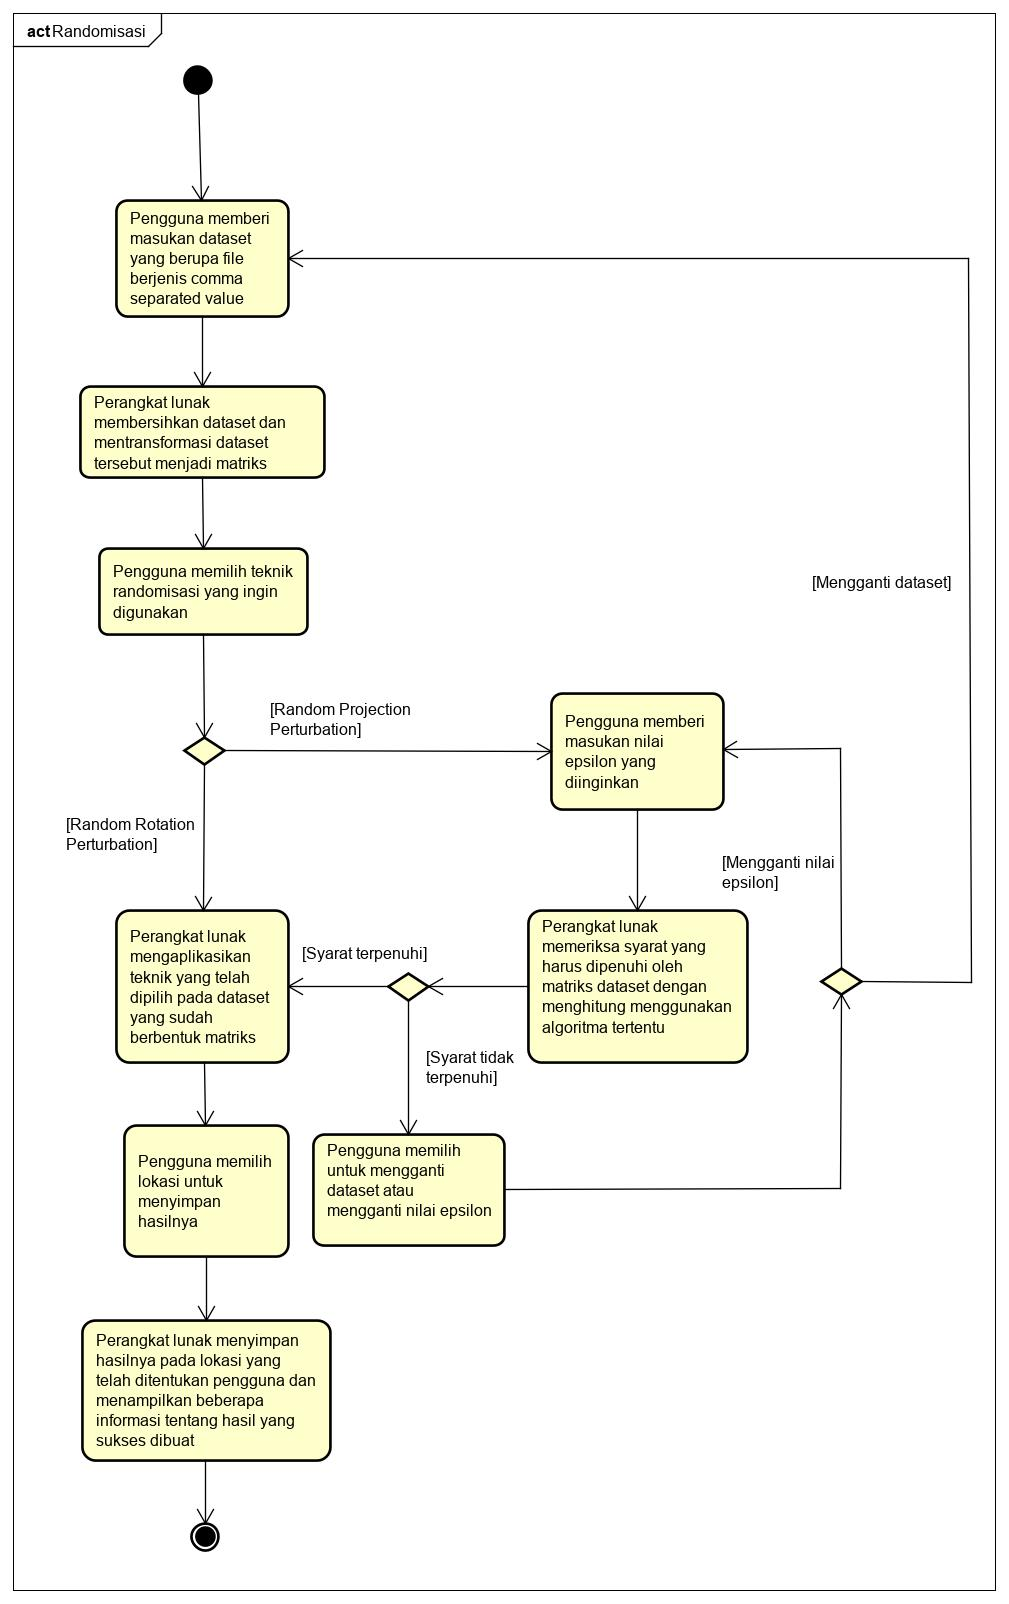
\includegraphics[scale=0.375]{activitydiagram}
    \caption{Diagram aktivitas perangkat lunak randomisasi}
    \label{fig:activitydiagram}
\end{figure}

Perangkat lunak randomisasi adalah perangkat lunak yang digunakan untuk memodifikasi data dengan metode \textit{Randomization}. Perangkat lunak ini akan memiliki fungsi untuk mengubah nilai setiap data yang dimasukan agar privasinya terjaga tetapi masih dapat dilakukan penambangan data. Algoritma \textit{Random Rotation Perturbation} dan \textit{Random Projection Perturbation} akan diimplementasikan pada perangkat lunak ini untuk fungsi utama yaitu mengubah nilai pada setiap data. Dengan mempertimbangkan studi literatur, analisis masalah, dan studi kasus yang telah dilakukan pada kedua teknik tersebut, perangkat lunak akan memiliki berbagai pilihan dan parameter yang pengguna harus masukan dan juga ada beberapa persyaratan atau batasan agar perangkat lunak ini berjalan dengan semestinya. Diagram aktivitas untuk perangkat lunak randomisasi dapat dilihat pada Gambar~\ref{fig:activitydiagram}. Berikut adalah penjelasan langkah-langkah pada diagram aktivitas tersebut.
\begin{enumerate}
    \item Pengguna memberikan masukan berupa dataset yang berupa dokumen berjenis \textit{comma-separated values} (CSV). Dokumen ini harus berisi tiap rekord pada barisnya dan tiap fitur pada kolomnya. Selain itu, pada baris pertama dalam dokumen tersebut harus berupa nama setiap fitur pada setiap kolomnya
    \item Perangkat lunak akan membersihkan dokumen yang berisi dataset tersebut dan mentransformasi datasetnya menjadi sebuah matriks. Matriks tersebut akan berisi nilai-nilai pada dataset saja tanpa nama kolom
    \item Pengguna memilih teknik randomisasi yang ingin digunakan antara \textit{Random Rotation Perturbation} dan \textit{Random Projection Perturbation}. Jika \textit{Random Projection Perturbation} yang dipiilih maka akan ada beberapa langkah yang harus dipenuhi yaitu sebagai berikut.
    \begin{enumerate}
        \item Pengguna memberi masukan nilai variabel \textit{epsilon} yang diinginkan. Variabel ini akan menentukan distorsi terburuk yang dapat terjadi pada hasil randomisasi dan menentukan nilai minimal variabel \textit{k}
        \item Perangkat lunak menghitung nilai minimal variabel \textit{k} lalu menampilkannya kepada pengguna dan memeriksa sebuah persyaratan yaitu apakah nilai nilai minimal variabel \textit{k} tersebut tidak melebihi dimensi dataset
        \item Jika persyaratan tidak terpenuhi maka pengguna harus memilih untuk mengganti datasetnya atau mengganti nilai variabel \textit{epsilon}
        \item Jika persyaratan terpenuhi maka berikutnya pengguna memberikan masukan nilai variabel \textit{k} yang diinginkan. Nilai yang diberikan pengguna harus lebih dari nilai minimal variabel \textit{k} yang sudah dihitung oleh perangkat lunak pada langkah sebelumnya
        \item Perangkat lunak memeriksa persyaratan teknik yaitu nilai variabel \textit{k} yang diberikan harus lebih kecil dari dimensi dataset dan lebih besar dari nilai minimal variabel \textit{k}.
        \item Jika persyaratan tidak terpenuhi maka pengguna harus mengganti nilai variabel \textit{k} kembali.
    \end{enumerate}
    \item Pengguna memilih untuk membuat matriks rotasi/proyeksi baru sesuai teknik yang dipilih atau pengguna dapat mengimpor matriks yang telah dibuat dan disimpan sebelumnya
    \item Berikut ini langkah-langkah tambahan yang harus dilakukan pengguna apabila pengguna memilih untuk membuat matriks rotasi/proyeksi baru
    \begin{enumerate}
        \item Pengguna memilih lokasi direktori pada komputer pengguna sebagai lokasi untuk menyimpan matriks rotasi/proyeksi yang akan dibuat
        \item Perangkat lunak membuat matriks rotasi/proyeksi baru dan menyimpan hasilnya pada lokasi yang telah dipiilih pengguna dalam bentuk dokumen berjenis CSV
    \end{enumerate}
    \item Berikut ini langkah-langkah tambahan yang harus dilakukan pengguna apabila pengguna memilih untuk mengimpor matriks rotasi/proyeksi yang pernah dibuat sebelumnya
    \begin{enumerate}
        \item Pengguna memilih matriks rotasi atau proyeksi sesuai teknik yang dipilih berupa dokumen berjenis CSV pada sebuah direktori komputer pengguna yang dipilih
        \item Perangkat lunak memeriksa dokumen CSV yang dipilih berisi matriks rotasi/proyeksi yang sesuai dengan dataset dan teknik randomisasi yang dipiilih
        \item Jika tidak sesuai maka pengguna harus memilih kembali matriks rotasi/proyeksi dengan benar
        \item Jika sudah sesuai dan memenuhi persyaratan maka perangkat lunak akan memproses dokumen CSV yang dipilih pengguna untuk menjadi matriks rotasi/proyeksi yang dapat dipakai untuk teknik randomisasi yang dipiilih
    \end{enumerate}
    \item Perangkat lunak mengaplikasikan teknik yang telah dipilih pada dataset yang sudah berbentuk matriks dengan memakai matriks rotasi/proyeksi yang telah dipilih
    \item Pengguna memilih lokasi direktori pada komputer pengguna untuk menyimpan hasil randomisasi dari teknik yang dipilih. Hasilnya adalah sebuah dokumen \textit{comma-separated values} yang berisi dataset yang telah dirandomisasi
    \item Perangkat lunak menyimpan hasilnya pada lokasi yang telah ditentukan pengguna dalam bentuk dokumen berjenis \textit{comma-separated values} dan menampilkan beberapa informasi tentang hasil yang sukses dibuat
\end{enumerate}

\subsection{Diagram Kelas}
\label{subsec:diagram-kelas}

\begin{figure}
    \centering
    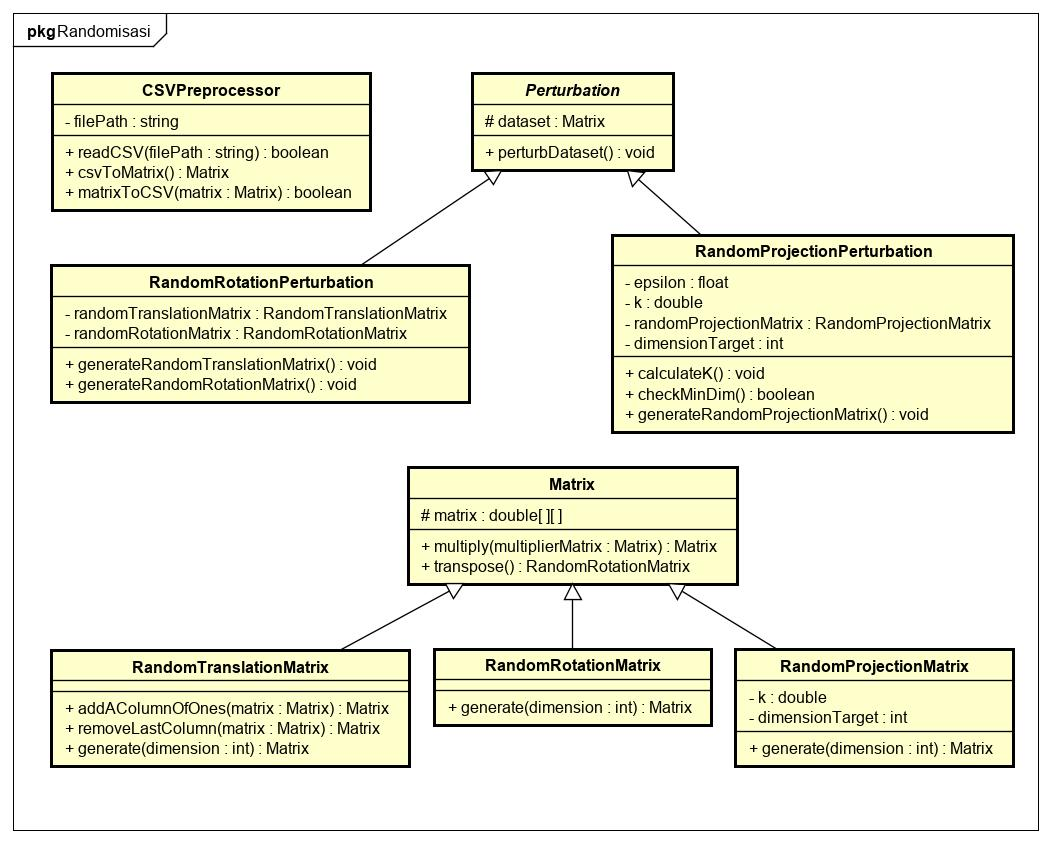
\includegraphics[scale=0.5]{classdiagram}
    \caption{Diagram kelas perangkat lunak randomisasi}
    \label{fig:classdiagram}
\end{figure}

Perancangan diagram kelas didasarkan pada analisis terhadap algoritma yang ingin diimplementasikan yaitu \textit{Random Rotation Perturbation} dan \textit{Random Projection Perturbation}, serta berdasarkan pada diagram aktivitas yang telah dibuat, dan dengan mempertimbangkan studi literatur, analisis masalah, dan studi kasus yang telah dilakukan pada kedua algoritma randomisasi yang ingin diimplementasikan. Detail dari diagram kelas perangkat lunak randomisasi pada Gambar~\ref{fig:classdiagram} adalah sebagai berikut.
\begin{itemize}
    \item Kelas \textit{Perturbation} adalah kelas abstrak yang akan di-\textit{extend} oleh kelas yang mengimplementasikan algoritma \textit{Random Rotation Perturbation} dan \textit{Random Projection Perturbation}. Kelas ini mempunyai sebuah atribut yaitu \textit{dataset} yang berfungsi untuk menyimpan dataset yang ingin dirandomisasi. Ada sebuah fungsi pada kelas ini yaitu \textit{perturbDataset} yang berfungsi untuk menerapkan teknik randomisasi pada dataset yang ingin dirandomisasi dengan kata lain atribut \textit{dataset}
    \item Kelas \textit{RandomRotationPerturbation} adalah kelas turunan dari kelas \textit{Perturbation} yang bertujuan untuk mengimplementasikan algoritma \textit{Random Rotation Perturbation}. Kelas ini memiliki dua tambahan atribut yaitu \textit{randomTranslationMatrix} dan \textit{randomRotationMatrix} yang masing-masing memiliki fungsi untuk menyimpan matriks translasi dan matriks rotasi. Ada dua buah fungsi tambahan juga pada kelas ini yaitu \textit{generateRandomTranslationMatrix} dan \textit{generateRandomRotationMatrix} yang masing-masing memiliki fungsi untuk membuat matriks translasi dan matriks rotasi baru.
    \item Kelas \textit{RandomProjectionPerturbation} adalah kelas turunan dari kelas \textit{Perturbation} yang bertujuan untuk mengimplementasikan algoritma \textit{Random Projection Perturbation}. Kelas ini memiliki tiga tambahan atribut yaitu \textit{epsilon}, \textit{minK}, dan \textit{K} yang masing-masing memiliki fungsi untuk menyimpan nilai variabel \textit{epsilon}, nilai minimal variabel \textit{k}, dan nilai variabel \textit{k} yang akan dipakai untuk menerapkan algoritma \textit{Random Projection Perturbation}. Ada dua buah fungsi tambahan juga pada kelas ini yaitu \textit{calculateMinK} dan \textit{checkValueK} yang masing-masing memiliki fungsi untuk menghitung nilai minimal variabel \textit{k} dan memeriksa persyaratan pada nilai atribut \textit{K}.
    \item Kelas \textit{Matrix} adalah kelas untuk merepresentasikan matriks dan menyimpan nilai-nilai pada setiap elemen matriks. Kelas ini memiliki sebuah atribut yaitu \textit{matrix} yang berfungsi untuk menyimpan setiap elemen matriks yang ada. Kelas ini juga memiliki dua buah fungsi yaitu \textit{multiply} dan \textit{transpose} yang masing-masing berfungsi untuk melakukan operasi perkalian dan transpose matriks yang akan digunakan untuk implementasi kedua algoritma teknik randomisasi
    \item Kelas \textit{RandomTranslationMatrix} adalah kelas yang mempunyai tujuan utama untuk membuat matriks translasi secara acak. Kelas ini adalah kelas statis sehingga tidak bisa diinstansiasi dan hanya memiliki atribut atau fungsi statis saja. Ada tiga buah fungsi statis yaitu \textit{addAColumnOfOnes}, \textit{removeLastColumn}, dan \textit{generate}. Fungsi \textit{addAColumnOfOnes} memiliki fungsi untuk menambahkan sebuah kolom yang pada setiap baris memiliki nilai berupa angka 1 kepada sebuah matriks. Fungsi \textit{removeLastColumn} memiliki fungsi untuk menghapus kolom terakhir pada suatu matriks. Fungsi \textit{generate} adalah fungsi yang bertujuan untuk membuat matriks translasi baru secara acak
    \item Kelas \textit{RandomRotationMatrix} adalah kelas yang mempunyai tujuan utama untuk membuat matriks rotasi secara acak. Kelas ini adalah kelas statis sehingga tidak bisa diinstansiasi dan hanya memiliki atribut atau fungsi statis saja. Hanya ada sebuah fungsi pada kelas ini yaitu \textit{generate} yang memiliki fungsi untuk membuat matriks rotasi baru secara acak
    \item Kelas \textit{RandomProjectionMatrix} adalah kelas yang mempunyai tujuan utama untuk membuat matriks proyeksi secara acak. Kelas ini adalah kelas statis sehingga tidak bisa diinstansiasi dan hanya memiliki atribut atau fungsi statis saja. Hanya ada sebuah fungsi pada kelas ini yaitu \textit{generate} yang memiliki fungsi untuk membuat matriks proyeksi baru secara acak
    \item Kelas \textit{CSVPreprocessor} adalah kelas untuk menangani masukan dataset berupa dokumen \textit{comma-separated values} yang akan direpresentasikan menjadi matriks. Kelas ini berguna untuk mengkonversi dokumen berjenis \textit{comma-separated values} menjadi matriks dan sebaliknya. Hanya ada sebuah atribut pada kelas ini yaitu \textit{filePath} yang berfungsi untuk menyimpan lokasi dokumen yang ingin diproses menjadi matriks. Ada tiga buah fungsi pada kelas ini yaitu \textit{readCSV}, \textit{csvToMatrix}, dan \textit{matrixToCSV} yang masing-masing berfungsi untuk membaca dokumen berjenis \textit{comma-separated values}, mengkonversi dokumen \textit{comma-separated values} menjadi matriks, dan mengkonversi matriks menjadi dokumen \textit{comma-separated values}.
    \item Kelas \textit{RotationMatrixPreprocessor} adalah kelas untuk menangani masukan matriks rotasi yang digabung dengan matriks translasi berupa sebuah dokumen \textit{comma-separated values} yang akan dikonversi menjadi dua buah matriks (rotasi dan translasi) dan sebaliknya. Ada dua buah fungsi pada kelas ini yaitu \textit{readCSV} dan \textit{saveToCSV}. Fungsi \textit{readCSV} berfungsi untuk membaca dokumen berjenis \textit{comma-separated values} untuk dikonversi menjadi matriks rotasi dan matriks translasi. Fungsi \textit{SaveToCSV} berfungsi untuk mengkonversi matriks rotasi dan matriks translasi menjadi sebuah dokumen berjenis \textit{comma-separated values}.
    \item Kelas \textit{ProjectionMatrixPreprocessor} adalah kelas untuk menangani masukan matriks proyeksi berupa sebuah dokumen \textit{comma-separated values} yang akan dikonversi menjadi sebuah matriks. Ada dua buah fungsi pada kelas ini yaitu \textit{readCSV} dan \textit{saveToCSV}. Fungsi \textit{readCSV} berfungsi untuk membaca dokumen berjenis \textit{comma-separated values} untuk dikonversi menjadi matriks proyeksi. Fungsi \textit{SaveToCSV} berfungsi untuk mengkonversi matriks proyeksi menjadi sebuah dokumen berjenis \textit{comma-separated values}.
\end{itemize}
